\chapter{Realisierung}\label{ch:realisierung}
In diesem Kapitel wird die tatsächliche Umsetzung der automatischen Datengenerierung für das \ac{CIF} thematisiert. Zunächst wird eine grundsätzliche Implementierung auf Basis des im vorangegangenen Kapitel beschriebenen Konzepts für die Equipment-Entität Chassis dargestellt. Das darauf folgende Unterkapitel \ref{sec:tdgmodule} beschäftigt sich mit der Erweiterung der Basisimplementierung zur Unterstützung von verschiedenen auch komplexeren Entitäten am Beispiel der Subequipment-Entität Module. Schließlich wird im Kapitel \ref{sec:tdgtelco} noch ein Konzept für eine mögliche künftige Implementierung von Telekommunikations-Entitäten, im Weiteren Telco-Entitäten genannt, vorgestellt.

\section{Realisierung der Testdatengenerierung für Equipment-Entitäten am Beispiel der Chassis}\label{sec:tdgchassis}
Equipment-Entitäten sind relativ einfache Entitäten, welche für sich alleinstehend in \textit{Command} platziert werden können. Sie benötigen keine weitere Objekte als Vorbedingungen, wie es bei kompelexeren Entitäten wie Modules oder den meisten Telco-Entitäten der Fall ist. Somit bieten sich Equipment-Entitäten für eine erste und möglichst simple Implementierung einer Datengenerierung an. Zwar gibt es in \textit{Command} eine Anzahl verschiedener Equipment-Entitäten, jedoch verhalten sich diese alle sehr ähnlich, sodass eine Implementierung für eine dieser Entitäten ohne großen Mehraufwand auf sämtliche Entitäten der Equipment-Kategorie ausgeweitet werden kann. Für die erste Implementierung wird sich konkret auf die Entität Chassis konzentriert.

\subsection{Struktureller Aufbau der Testdatengenerierung}\label{subsec:tdgStruktur}
In dem in Kapitel \ref{ch:sollzustand} erarbeiteten Konzept bleibt die Frage nach dem tatsächlichen strukturellen Aufbau der Testdatengenerierung offen. Auch ohne konkrete Erwähnung wird allerdings klar, dass eine Unterteilung des Prozesses in verschiedene Klassen sinnvoll und nötig ist, um das Projekt möglichst übersichtlich zu halten. Für die Strukturierung der Datengenerierung wird sich in erster Linie an den in Kapitel \ref{sec:autotestsfnt} erwähnten Vorgaben der \textit{FNT} Qualitätssicherungs-\ac{CoP} orientiert, da die automatische Testdatengenerierung als Teil des automatisierten Testprojekts \enquote{CIF Automated Tests} den Firmenstandards und -richtlinien im Bereich der Softwaretests genügen soll.

Konkret bedeutet dies, dass die Testdatengenerierung fernab der sich im Pfad \textit{src/test/java} befindlichen Testklassen in eigene Klassen im Pfad \textit{src/main/java} ausgelagert wird. In der eigentlichen Testmethode der \textit{setUpEnvironment}-Testsuite sollen möglichst nur Methodenaufrufe getätigt werden und keinerlei Logik zur Generierung der Testdaten implementiert werden. Dies geschieht abseits der Tests in der Klasse \textit{DataGeneratorSteps}, welche sich mit bereits existierenden \textit{Step}-Klassen im Package \textit{com.fntsoftware.api.steps} befindet. In den Testmethoden wird also lediglich die Methode \textit{setUpHardwareTestData()} in der eben erwähnten Klasse aufgerufen, welche alle weiteren logischen Schritte einleitet und zu einem über \textit{JUnit-Assertions} prüfbaren Ergebnis führt.

Um die Klasse \textit{DataGeneratorSteps} ebenfalls möglichst übersichtlich zu halten, wird der Kern der Datengenerierung - im Konzept beschrieben in Schritt 4. bis 7. - erneut in eigene Klassen ausgelagert. Hierfür wird ein neues Package erstellt, welches im Projekt über den Pfad \textit{com.fntsoftware.api.datagenerator} zu finden ist. In diesem Package befindet sich zum Einen die Klasse \textit{DataGeneratorUtils}, welche Utility-Methoden zum Generieren von Werten enthält, zum Anderen aber auch die Klasse \textit{DataGenerator}. Letztere enthält mit der Methode \textit{generateTestData()} die Logik für das Generieren von Basisobjekten und den eigentlichen Testobjekten ausgehend davon.

\begin{figure}[h]
    \centering
    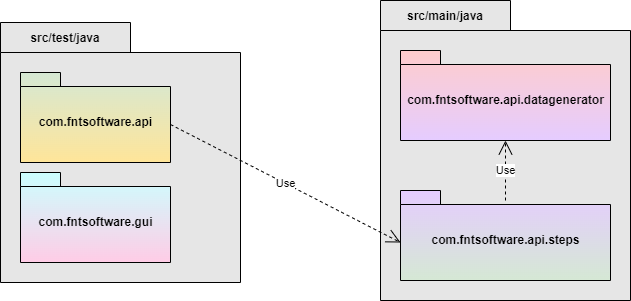
\includegraphics[width=.8\textwidth]{package-struktur.drawio.png}
    \caption{Aufbau der relevanten Packages im Testprojekt}
\end{figure}

\subsection{Erstellen und Parsen der Konfigurationsdateien}\label{subsec:config}
Bevor eine Realisierung der eigentlichen Datengenerierung erfolgen kann, müssen die Konfigurationsdateien definiert werden. Es wurde sich für hierbei für das \ac{CSV}-Format entschieden, da \ac{CSV}-Dateien in Programmen wie \textit{Microsoft Excel} in Tabellenform geöffnet und auch dort direkt bearbeitet werden können. \cite{excel:2022} Dies bietet die Möglichkeit, die Konfigurationsdateien gleichzeitig gewissermaßen als Dokumentation zu verwenden, da sie auch beschreiben, welche Deltafälle und Entitäten in der Datengenerierung bereits umgesetzt sind. Im Folgenden sind sowohl die Konfigurationsdatei für die Deltafälle als auch die Datei für die Entitäten beispielhaft zunächst in der eigentlichen \ac{CSV}- und daraufhin auch in ihrer Tabellenansicht dargestellt und werden jeweils näher erläutert.

\begin{lstlisting}[caption=Konfigurationsdatei für Deltafälle im CSV-Format, label=deltaConfig,language=csv,basicstyle=\scriptsize\ttfamily]
Delta Case;NMS_Record;Command_Record;Planned_Create_Record;Planned_Delete_Record
CREATE;nms;;;
UPDATE;nms;command;;
DELETE;;command;;
UPDATE_TYPE;nms;command;;
PLANNED_CREATE;nms;;planningCreate;
PLANNED_CREATE_NOP;;;planningCreate;
PLANNED_CREATE_BUT_WITH_DIFFERENT_TYPE;nms;;planningCreate;
PLANNED_DELETE;;command;;planningDelete
PLANNED_DELETE_NOP;nms;command;;planningDelete
PLANNED_DELETE_WITH_CREATE;nms;command;;planningDelete
PLANNED_DELETE_WITH_PLANNED_CREATE_BUT_WITH_DIFFERENT_TYPE;nms;command;planningCreate;planningDelete
PLANNED_DELETE_WITH_PLANNED_CREATE;nms;command;planningCreate;planningDelete
PLANNED_DELETE_WITH_PLANNED_CREATE_NOP;nms;command;planningCreate;planningDelete
PLANNED_DELETE_WITH_PLANNED_CREATE_NOP_DELETION;;command;planningCreate;planningDelete
\end{lstlisting}

\begin{sidewaystable}
\begin{center}
    \scriptsize
    \begin{tabular}{| >{\raggedright\arraybackslash}m{39.5em} | >{\raggedright\arraybackslash}m{5em} | >{\raggedright\arraybackslash}m{7em} | >{\raggedright\arraybackslash}m{10em} | >{\raggedright\arraybackslash}m{10em} |}
        \hline
         Delta Case & NMS\_Record & Command\_Record & Planned\_Create\_Record & Planned\_Delete\_Record \\ 
         \hline\hline
         CREATE & nms & & & \\ 
         \hline
         UPDATE & nms & command & & \\  
         \hline
         DELETE & & command & & \\ 
         \hline
         UPDATE\_TYPE & nms & command & & \\ 
         \hline
         PLANNED\_CREATE & nms & & planningCreate & \\ 
         \hline
         PLANNED\_CREATE\_NOP & & & planningCreate & \\ 
         \hline
         PLANNED\_CREATE\_BUT\_WITH\_ DIFFERENT\_TYPE & nms & & planningCreate & \\ 
         \hline
         PLANNED\_DELETE & & command & & planningDelete \\ 
         \hline
         PLANNED\_DELETE\_NOP & nms & command & & planningDelete \\ 
         \hline
         PLANNED\_DELETE\_WITH\_ CREATE & nms & command & & planningDelete \\ 
         \hline
         PLANNED\_DELETE\_WITH\_PLANNED\_CREATE\_BUT\_WITH\_DIFFERENT\_TYPE & nms & command & planningCreate & planningDelete \\ 
         \hline
         PLANNED\_DELETE\_WITH\_PLANNED\_CREATE & nms & command & planningCreate & planningDelete \\ 
         \hline
         PLANNED\_DELETE\_WITH\_PLANNED\_CREATE\_NOP & nms & command & planningCreate & planningDelete \\ 
         \hline
         PLANNED\_DELETE\_WITH\_PLANNED\_CREATE\_NOP\_DELETION & & command & planningCreate & planningDelete \\ 
        \hline
    \end{tabular}
    \caption{Konfigurationsdatei für Deltafälle in Tabellenform}\label{tab:deltaConfig}
\end{center}
\end{sidewaystable}

Das \ac{CSV}-Format erlaubt optional die Verwendung der ersten Zeile als Kopfzeile. Dies ermöglicht eine Verbesserung der Übersichtlichkeit und der Verständlichkeit insbesondere in der Tabellenform. Die Spalte \enquote{Delta Case} beinhaltet alle von den Equipment-Entitäten unterstützten und zu testenden Deltafälle. Die weiteren Spalten legen fest, in welche Tabellen Objekte platziert werden müssen, um einen Deltafall zu erfüllen. Ein Eintrag in der Spalte \enquote{NMS\_Record} bedeutet beispielsweise, dass ein \ac{NMS}-Objekt generiert und in die zur Entität gehörende \ac{NMS}-Tabelle gefüllt werden muss. Die Spalten \enquote{Planned\_Create\_ Record} und \enquote{Planned\_Delete\_Record} drücken aus, dass Objekte mit aktiviertem Planning Protocol erstellt oder gelöscht werden müssen. Zu erwähnen ist, dass nur diese Konfiguration nicht ausreicht, um zwischen allen Deltafällen zu differenzieren. Wie in der Tabelle zu sehen, besitzen manche Deltafälle dieselben Anforderungen in Hinsicht auf \ac{NMS}- und \textit{Command}-Tabellen. Dies liegt daran, dass die soeben beschriebene Konfigurationsdatei keine Attributsanforderungen der Deltafälle berücksichtigt. Bei einigen Deltafälle, beispielsweise \enquote{PLANNED\_CREATE\_BUT\_WITH\_DIFFERENT\_TYPE}, müssen sich die Objekte in den verschiedenen Tabellen in bestimmten Attributwerten unterscheiden. Im genannten Fall würde das Fehlen dieser Attributsunterschiede dazu führen, dass der Deltafall als \enquote{PLANNED\_CREATE} erkannt wird, denn hierfür werden Objekte in dieselben Tabellen platziert, ohne sich dabei in ihren Attributwerten zu unterscheiden.

\newpage
Auch bei der Entitäts- beziehungsweise Testdaten-Konfigurationsdatei wird die erste Zeile wieder als separate Kopfzeile verwendet und es werden analog zur Deltafall-Konfiguration in Listing \ref{deltaConfig} und Tabelle \ref{tab:deltaConfig} sämtliche Deltafälle in der ersten Spalte dokumentiert. Alle weiteren Spalten dienen in dieser Konfiguration allerdings dazu, Entitäten für die Testdatengenerierung zu definieren. Ein Eintrag des Entitätsnamens in einer Zeile bedeutet hierbei, dass für diese Entität und den Deltafall in ebendieser Zeile Testdaten generiert werden sollen.

\begin{lstlisting}[caption=Konfigurationsdatei für Entitäten im CSV-Format, label=entityConfig,language=csv,basicstyle=\footnotesize\ttfamily]
Delta Case;Chassis;...
CREATE;Chassis;...
UPDATE;Chassis;...
DELETE;Chassis;...
UPDATE_TYPE;Chassis;...
PLANNED_CREATE;Chassis;...
PLANNED_CREATE_NOP;Chassis;...
PLANNED_CREATE_BUT_WITH_DIFFERENT_TYPE;Chassis;...
PLANNED_DELETE;Chassis;...
PLANNED_DELETE_NOP;Chassis;...
PLANNED_DELETE_WITH_CREATE;Chassis;...
PLANNED_DELETE_WITH_PLANNED_CREATE_BUT_WITH_DIFFERENT_TYPE;Chassis;..
PLANNED_DELETE_WITH_PLANNED_CREATE;Chassis;...
PLANNED_DELETE_WITH_PLANNED_CREATE_NOP;Chassis;...
PLANNED_DELETE_WITH_PLANNED_CREATE_NOP_DELETION;Chassis;...
\end{lstlisting}

\begin{table}[h]
\begin{center}
    \scriptsize
    \begin{tabular}{| p{42em} | m{3em} | m{1em} |}
        \hline
         Delta Case & Chassis & \ldots \\ 
         \hline\hline
         CREATE & Chassis & \ldots \\ 
         \hline
         UPDATE & Chassis & \ldots \\  
         \hline
         DELETE & Chassis & \ldots \\ 
         \hline
         UPDATE\_TYPE & Chassis & \ldots \\ 
         \hline
         PLANNED\_CREATE & Chassis & \ldots \\ 
         \hline
         PLANNED\_CREATE\_NOP & Chassis & \ldots \\ 
         \hline
         PLANNED\_CREATE\_BUT\_WITH\_ DIFFERENT\_TYPE & Chassis & \ldots \\ 
         \hline
         PLANNED\_DELETE & Chassis & \ldots \\ 
         \hline
         PLANNED\_DELETE\_NOP & Chassis & \ldots \\ 
         \hline
         PLANNED\_DELETE\_WITH\_ CREATE & Chassis & \ldots \\ 
         \hline
         PLANNED\_DELETE\_WITH\_PLANNED\_CREATE\_BUT\_WITH\_DIFFERENT\_TYPE & Chassis & \ldots \\ 
         \hline
         PLANNED\_DELETE\_WITH\_PLANNED\_CREATE & Chassis & \ldots \\ 
         \hline
         PLANNED\_DELETE\_WITH\_PLANNED\_CREATE\_NOP & Chassis & \ldots \\ 
         \hline
         PLANNED\_DELETE\_WITH\_PLANNED\_CREATE\_NOP\_DELETION & Chassis & \ldots \\ 
        \hline
    \end{tabular}
    \caption{Konfigurationsdatei für Entitäten in Tabellenform}\label{tab:entityConfig}
\end{center}
\end{table}

Die dargestellten \ac{CSV}-Dateien können nun geparst und für den Datengenerierungsprozess verwendbar gemacht werden. Hierfür wird jeweils eine eigene statische Methode in der Klasse \textit{RessourceProvider} definiert, welche die Inhalte der Dateien auf Objekte vom Typ \colorbox{background}{\lstinline{LinkedHashMap<String, List<String>>}} mappt und diese zurückgibt. Der folgende Codeausschnitt zeigt eine dieser Methoden für das Parsen der Entitäts- oder auch Testdatenkonfiguration. 

\begin{lstlisting}[caption=Methode zum Parsen und Mappen der Testdatenkonfiguration, label=testdataParse,language=Java]
public static LinkedHashMap<String, List<String>> getTestDataConfiguration(String path)
		throws IOException {
	LinkedHashMap<String, List<String>> map = new LinkedHashMap<String, List<String>>();

	List<String[]> collect = Files.lines(getConfigRessourceFile(path).toPath()).map(line -> line.split(",|;"))
			.collect(Collectors.toList());

	for (int i = 1; i < collect.size(); i++) {
		for (int j = 1; j < collect.get(i).length; j++) {
			if (!collect.get(i)[j].equals("")) {
				if (!map.containsKey(collect.get(i)[j])) {
					map.put(collect.get(i)[j], new ArrayList<>(List.of(collect.get(i)[0])));
				} else {
					map.computeIfAbsent(collect.get(i)[j], k -> new ArrayList<String>()).add(collect.get(i)[0]);
				}
			}
		}
	}
}
\end{lstlisting}

Die seit Java 8 vorhandene Stream-\ac{API} ermöglicht das einfache zeilenweise Lesen einer über einen Pfad angegebenen Datei und liefert diese als String-Stream zurück. Die einzelnen Zeilenstrings können mithilfe der Methode \textit{split()} an den \ac{CSV}-Separatoren getrennt und so die Werte schließlich zu einer Liste gemappt werden, welche die einzelnen Zeilen als String-Arrays in ihre separaten Werte getrennt speichert. Im nächsten Schritt wird über diese Liste mithilfe von zwei verschachtelten Schleifen iteriert. Die äußere Schleife dient zur Betrachtung der Zeilen, also der kompletten String-Arrays, während die innere Schleife über die Werte der jeweils betrachteten Arrays verläuft. Hierbei steht an erster Stelle im Array immer der Deltafall, weshalb zur Filterung der Entitäten die Werte ab Index 1 des Arrays gelesen werden. Enthält das Array am momentanen Index einen Wert, also einen Entitätsnamen, wird ein Key-Value-Paar zu einer \textit{LinkedHashMap} hinzugefügt, wobei der Entitätsname als Key und und der bisher ignorierte zugehörige Deltafall als Wert in Form einer \textit{ArrayList} fungiert. Ist die Entität bereits in der Map enthalten, wird statt dem Hinzufügen eines neuen Key-Value-Paars die \textit{ArrayList} von Deltafällen für die Entität um den zur momentan betrachteten Zeile gehörenden Fall erweitert. Nachdem beide Schleifen vollständig durchlaufen sind, enthalten die Keys der \textit{LinkedHashMap} alle Entitäten und die Values für jede Entität eine Liste mit genau jenen Deltafällen, für welche die Entität in der Konfigurationsdatei definiert wurde. Der Aufruf der \textit{getTestDataConfiguration()}-Methode erfolgt als erster Schritt direkt zu Beginn der Testmethode in der \textit{setUpEnvironment}-Testsuite. Die hieraus erhaltene \textit{LinkedHashMap} mit der Konfiguration wird als Parameter an die Methode \textit{setUpHardwareTestData()} der \textit{DataGeneratorSteps}-Klasse übergeben.

Das Vorgehen beim Parsen und Mappen der Deltafall-Konfigurationsdatei verläuft im Grunde ähnlich zum beschriebenen Ablauf, weshalb auf dieses nicht näher eingegangen wird. Die hierzu implementierte Methode \textit{getDeltaSpecifications()} wird jedoch erst zu Beginn der \textit{setUpHardwareTestData()}-Methode aufgerufen.

\subsection{Iterieren über die Entitäten}\label{subsec:iterationEntities}
Mit Beginn der äußeren Iterationsebene beginnt auch die eigentliche Testdatengenerierung. Diese Ebene findet in der \textit{setUpHardwareTestData()}-Methode statt, welche die \textit{HashMap}-Repräsentation der Testdatenkonfiguration als Methodenparameter übergeben bekommt, sodass über deren Einträge mithilfe der Java-Utility-Methode \textit{HashMap.entrySet()} iteriert werden kann. Zwar sind Java-Maps eigentlich nicht mit \textit{foreach}-Schleifen kompatibel, jedoch liefert diese Methode eine Ansicht aller Mappings in einer Java-Map als \textit{Entry}-Objekte in einem Set, welches wiederum das Verwenden einer \textit{foreach}-Schleife ermöglicht. So kann ohne Schleifenzähler Eintrag für Eintrag über die Map iteriert werden und gleichzeitig über das \textit{Entry}-Objekt für den betrachteten Eintrag sowohl auf den Key als auch den Value durch Getter-Methoden zugegriffen werden.

Für die weitere Datengenerierung wird der Entitätsname in verschiedenen Varianten benötigt. Der eigentliche Name der Entität, welcher aus dem Key des \textit{Entry}-Objekts gelesen werden kann, unterscheidet sich bei manchen Entitäten vom Namen in der Datenbank oder in \ac{BGE}-\ac{REST}-Pfaden. Nach umfassender Analyse der Testdaten stellte sich beispielsweise heraus, dass die Entität Client in den \ac{BGE}-Operationen \enquote{Terminal} heißt. Zwar würde dies in einer ersten Implementierung zu keinem Fehler führen, da sich die Namen beim Chassis nicht unterscheiden, jedoch ist mit Hinblick auf die Skalierbarkeit der Testdatengenerierung eine solche Besonderheit von Beginn an zu berücksichtigen. Es werden also für die betrachtete Entität in der äußeren Schleife drei separate String-Variablen mit den möglichen Varianten der Entitätsnamen definiert:

\begin{itemize}
    \item \textbf{entityName.} Der reguläre Name der Entität, welcher auch durch den Key des momentanen \textit{Entry}-Objekts repräsentiert wird.
    \item \textbf{entityId.} Die \textit{entityId} wird aus der Entitätskonfiguration (s. Kapitel \ref{subsec:attributes}) ausgelesen und dient der Verwendung in \ac{REST}-Pfaden.
    \item \textbf{entityTableName.} Dieser Name entspricht dem in der Datenbank verwendeten Entitätsnamen und kann ebenfalls aus der Entitätskonfiguration erhalten werden.
\end{itemize}

\subsection{Abfragen der Attribute}\label{subsec:attributes}
Der nächste logische Schritt im Programmablauf stellt die Abfrage der Entitätsattribute dar. Diese bieten die Grundlage zur darauffolgenden Erstellung der Basisobjekte, um daraus valide Testdaten generieren zu können. Wie schon in Kapitel \ref{subsec:konzept} erwähnt, können die \ac{NMS}-Attributkonfigurationen über die \ac{BGE} abgefragt werden. Dies geschieht in zwei Schritten:

\begin{enumerate}
    \item \textit{/rest/entity/cifEntityConfiguration/query}
    \item \textit{/rest/entity/cifEntityConfiguration/\{entityElid\}/QueryCifAttributeConfiguration}
\end{enumerate}

Im ersten Schritt wird die Entitätskonfiguration abgefragt. Hierfür wird an den \ac{REST}-Endpunkt eine Anfrage gesendet, welche den \textit{entityName} in ihrem \ac{JSON}-Body als sogenannte \enquote{Restriction}, also Sucheinschränkung, beinhaltet. Zurückgeliefert wird eine Antwort in \ac{JSON}-Form, welche im Folgenden für die Entität \enquote{Chassis} dargestellt ist.

\begin{lstlisting}[caption=Entitätskonfiguration des Chassis in JSON-Form, label=entityConfigResponse,language=json]
{
    "commandTableName": "STCDEV_CHASSIS",
    "elid": "QTSEUUSWNANYA8",
    "active": "Y",
    "commandEntityId": "CHASSIS",
    "nmsTableName": "STFIFC_NMS_CHASSIS",
    "synchronizationOrder": 9,
    "deltaSqlFilename": "HardwareDelta.sql",
    "remark": "Intermediate table to keep NMS chassis data, loaded from external system",
    "dynamic": "N",
    "entityName": "Chassis"
}
\end{lstlisting}

Für das Abfragen der Attributkonfigurationen wird lediglich die \ac{Elid} der Entität benötigt, jedoch können die Attribute \textit{commandEntityId} und \textit{commandTableName} für die im vorigen Kapitel angesprochenen String-Variablen \textit{entityId} und \textit{entityTableName} verwendet werden.

Um die Attributkonfigurationen zu erhalten, muss die zweite \ac{REST}-Anfrage die \ac{Elid} der Entität direkt im Pfad beinhalten. Hierfür bietet das im Testprojekt bereits verwendete \textit{RESTeasy}-Framework die Möglichkeit, für Methoden, welche für \ac{REST}-Anfragen verwendet werden sollen, Pfadparameter zu definieren. Hierfür werden normale Methodenparameter mit der Annotation \textit{@PathParam} versehen und so bei Ausführung des \ac{REST}-Aufrufs direkt in die im Pfad mit geschweiften Klammern markierte Stelle eingesetzt. Für Chassis ergibt sich so beispielsweise der folgende Pfad: 
\begin{center}
    \textit{[...]/cifEntityConfiguration/QTSEUUSWNANYA8/QueryCifAttributeConfiguration}
\end{center}

Eine Anfrage an diesen \ac{REST}-Endpunkt liefert daraufhin ein \ac{JSON}-Array bestehend aus den Konfigurationen für alle \ac{NMS}-Attribute, welche die Entität besitzt. Dieses \ac{JSON}-Array kann mithilfe der Java-Bibliothek \textit{Jackson} zu einer Java-Liste deserialisiert und, gemeinsam mit den Entitätsnamen und der Delta-Spezifikation, an die \textit{generateTestData()}-Methode in der Klasse \textit{DataGenerator} übergeben werden.

\subsection{Erstellen von Basisobjekten}\label{subsec:baseObjects}
Dem Erstellen von Basisobjekten fällt in der Testdatengenerierung ein besonders hoher Stellenwert zu, da diese im Grunde dafür sorgen, dass die Testdaten überhaupt valide generiert und in \textit{Command} erstellt werden können. Das Verfahren zur Erstellung dieser Objekte soll dabei so generisch wie möglich gestaltet werden, sodass bei Erweiterungen der automatischen Testdatengenerierung keine größeren Änderungen mehr vonnöten sind. 

Dies wird einerseits durch das Verwenden der \ac{CIF}-Attributkonfigurationen realisiert. Diese besitzen einen generischen Aufbau und können für jede Hardware-Entität auf dieselbe Art über die \ac{BGE} abgefragt werden. Lediglich der Entitätsname ist ausschlaggebend für die zurückgelieferten Attribute und die Konfigurationen für sämtliche Attribute sind gleich aufgebaut. Andererseits kann eine möglichst generische Basisobjekterstellung durch ein generell generisch aufgebautes Testdatenobjekt erreicht werden. Dies bedeutet konkret, dass für die verschiedenen Entitäten keine individuellen Klassen verwendet werden, sondern jedes generierte Objekt durch eine simple \textit{HashMap} dargestellt wird. Deren Keys bilden die Attributnamen ab und die zugehörigen Values enthalten die entsprechenden Attributwerte. Diese einfache Struktur erlaubt es, alle möglichen Entitäten ohne jedwede angepasste Objektklasse flexibel zu verwalten und jederzeit nur durch das Hinzufügen eines Key-Value-Paars zu modifizieren. Mithilfe einer selbst implementierten \textit{toString()}-Methode können diese generischen Testdaten-\textit{HashMap}-Objekte daraufhin für die Verwendung in \ac{BGE}-Anfragen zu \ac{JSON}-Strings konvertiert werden. 

Für das Erstellen dieser generischen Basisobjekte müssen zunächst Informationen zur im betrachteten Testzyklus erstellten Zone und zu den auf der \textit{Command}-Instanz vorhandenen Gerätetypen, auch Device Master genannt, aus \textit{Command} abgefragt werden. Hierdurch können diese Werte für alle weiteren generierten Objekte wiederverwendet werden, ohne für jedes neu generierte Objekt eigene \ac{BGE}- oder Datenbankabfragen zu stellen. 

Die Zoneninformationen können über eine einfache \ac{BGE}-Abfrage erhalten werden, die Device Master sind auf diesem Weg jedoch nicht einsehbar. Um alle existierenden Device Master für eine Entität zu sammeln, wird stattdessen eine Datenbankabfrage durchgeführt. Sämtliche Device Master für Equipments und auch Subequipments sind in der Tabelle \textit{STCSPC\_DEVICE} festgehalten, wobei die Spalte \textit{CONFIG\_TABLE\_NAME} verwendet wird, um die zugehörige Entität zu identifizieren. Der Wert \textit{STCDEV\_CHASSIS} bezeichnet dabei beispielsweise Device Master für die Entität Chassis. Generell wird dieser Wert durch den \textit{entityTableName} abgebildet. Nach der Datenbankabfrage wird ein Device Master für das Basisobjekt herausgesucht und die restlichen Device Master als Liste in einer Variablen gespeichert, sodass für weitere Objekte, welche bei bestimmten Deltafällen vom Basisobjekt abweichende Device Master benötigen, ein einfacher Zugriff ermöglicht wird.

Nachdem Device Master und Informationen zu den Zonen abgefragt wurden, können die Basisobjekte erstellt werden. Zuerst wird das \ac{NMS}-Basisobjekt erstellt, da hierfür das direkte Verwenden der Attributkonfigurationen ausreicht. Alle Attribute mit Wert \colorbox{background}{\lstinline{\"synchronizeToCommand\": \"Y\"}} werden in der Basisobjekt-Map als Keys mit leeren Werten als Platzhalter hinzugefügt. Außerdem müssen die Attribute \textit{groupingId}, \textit{commandType} und \textit{commandZoneId} aus der Konfiguration übernommen werden, obwohl diese nicht zur Synchronisation markiert sind. Sie werden allerdings für die korrekte Ausführung der Tests benötigt.

\begin{lstlisting}[caption=Methode zum Erstellen eines NMS-Basisobjekts, label=nmsBaseRecord,style=Javastyle]
protected Map<String, String> createNmsBaseRecord(List<CifAttributeConfigurationResponse> attribConfig) {
	HashMap<String, String> recordBase = new HashMap<>();

	for (CifAttributeConfigurationResponse attrib : attribConfig) {
		if ("Y".equals(attrib.getSynchronizeToCommand()) || "GROUPING_ID".equals(attrib.getAttrName())
				|| "COMMAND_TYPE".equals(attrib.getAttrName()) || "COMMAND_ZONE_ID".equals(attrib.getAttrName())) {
			if (attrib.getAttrName().equalsIgnoreCase("SOURCE_SYSTEM")) {
				recordBase.put("nmsSourceSystem", null); // necessary because the attribute is named differently in
															// the
															// Cif Attribute Configuration
			} else {
				recordBase.put(DataGeneratorUtils.makeCamelCase(attrib.getAttrName()), null);
			}
		}
	}
	return recordBase;
}
\end{lstlisting}

Nach dem \ac{NMS}-Basisobjekt wird das \textit{Command}-Basisobjekt erstellt. Dieses ist nicht ohne Weiteres aus der Attributkonfiguration zu erstellen, da die Attribute lediglich \ac{NMS}-Objekte zuverlässig beschreiben. Zwar können auch hier zumindest die Attribute aus der Attributkonfiguration übernommen werden, welche als zur Synchronisation relevant markiert sind - besitzen sie auch einen Wert für das Attribut \textit{commandAttribName}, so kann dieser Wert für das Basisobjekt übernommen werden. Jedoch fehlen danach immer noch Attribute, welche zunächst nicht identifizierbar sind. Um diese dennoch zu vervollständigen, wird wie folgt vorgegangen:

\begin{enumerate}
    \item Das \textit{Command}-Basisobjekt wird über die \ac{BGE} erstellt. Ist dieses noch unvollständig, liefert diese Operation einen Fehlercode und eine Fehlernachricht zurück.
    \item Die Fehlernachricht enthält Rückschlüsse auf das noch fehlende Attribut. Sie wird analysiert und das Attribut zum Basisobjekt hinzugefügt.
    \item Wurde in 1. ein Fehler produziert, dann wiederhole diese Schritte. Ansonsten war die Erstellung des Basisobjekts erfolgreich, das Objekt also valide, und es wird wieder aus \textit{Command} gelöscht.
\end{enumerate}

\begin{lstlisting}[caption=Vorgehen zum Vervollständigen des \textit{Command}-Basisobjekts, label=commandBaseRecord,style=Javastyle]
do {
    record.addRecord(commandBaseRecord);
    response = createObjectInCommand(sessionId, record.toCommandStrings().get(0));
    responsemapper = BaseApiBGE.getMapper().readValue(response.readEntity(String.class),
            new TypeReference<BgeQueryResponse<BgeCreateObjectResponse>>() {
            });
    if (responsemapper.getStatus().getErrorCode() != 0) {
        String msg = responsemapper.getStatus().getMessage();
        String missingAttributeName = DataGeneratorUtils.findMissingAttribute(msg);
        String missingAttributeValue = generateValue("", missingAttributeName.toLowerCase(), sessionId);
        commandBaseRecord.put(missingAttributeName, missingAttributeValue);
        record.clearRecords();
    } else {
        // delete checkRecord
        restOperations.getCommandPostconditionRestOperations().deleteCommandObject(this.entityId,
                responsemapper.getReturnData().get(0).getElid(), sessionId, "{}");
    }
} while (responsemapper.getStatus().getErrorCode() != 0);
\end{lstlisting}

\subsection{Iterieren über die Deltafälle}\label{subsec:iterationDeltacases}
Nachdem valide Basisobjekte erstellt wurden, können in der mittleren und inneren Iterationsebene die Testdaten für die Deltafälle generiert werden. Die mittlere Schleife dient hierbei zur Iteration über die in der Testdatenkonfiguration definierten Liste mit den zu betrachtenden Deltafällen für die Entität. Bevor in die innere Schleife zur Wertegenerierung fortgeschritten werden kann, wird der Deltafall mit den konfigurierten Deltafällen aus der Deltafall-Spezifikation abgeglichen, damit auch nur für korrekt eingetragene Deltafälle Daten generiert werden. Wird der Deltafall nicht erkannt, kommt es zum Werfen einer Exception mit der entsprechenden Fehlermeldung: \enquote{[...] is not a valid Delta Case!}

Sind alle Deltafälle für die Entität durchlaufen, wird die Schleife verlassen und die bis dorthin generierten Daten an die aufrufende Methode \textit{setUpHardwareTestData()} in der Klasse \textit{DataGeneratorSteps} zurückgegeben.

\subsection{Iterieren über die Testobjekttypen}\label{subsec:iterationObjectTypes}
In der inneren Iterationsebene wird für den in der mittleren Schleife betrachteten Deltafall über die Objekttypen iteriert, welche in der Deltafall-Spezifikation festgelegt sind. Um die einzelnen Typen zu unterscheiden, kommt eine \textit{switch-case}-Verzweigung zum Einsatz. Der erste Objekttyp, der betrachtet und, sofern benötigt, generiert wird, ist immer \enquote{nms}. Für diesen Typ wird als Referenz das \ac{NMS}-Basisobjekt verwendet und dabei Attribut für Attribut ein Wert generiert und dem zu konstruierenden neuen Testobjekt hinzugefügt. Auf die Wertegenerierung wird im nächsten Unterkapitel näher eingegangen.

Das Generieren eines neuen Testobjekts vom Typ \enquote{command} oder auch \enquote{planningCreate} verläuft analog zum oben beschriebenen Vorgehen, jedoch wird hier das \textit{Command}-Basisobjekt als Referenz verwendet, sollte vor dem zu erstellenden Objekt noch kein weiteres erstellt worden sein. Ist dies allerdings nicht der Fall, wird statt des Basisobjekts das zuvor generierte Testobjekt als Referenz verwendet. Hierfür wird im ersten Schleifendurchgang das dort generierte Objekt einer \textit{referenceRecord}-Variablen zugewiesen. In der \textit{switch-case}-Verzweigung findet eine Überprüfung des Schleifenzählers statt - befindet sich die Schleife nicht in ihrer ersten Iteration, werden nicht mehr Attribut für Attribut am Basisobjekt entlang Werte generiert, sondern mithilfe der Methode \textit{generateSimilarRecord()} anhand des existierenden \textit{referenceRecord}-Objekts ein neues Objekt erstellt, welches die meisten Werte des Referenzobjekts übernimmt. Hiermit kann gewährleistet werden, dass zusammengehörige Testobjekte, wie es die einzelnen Objekte für einen Deltafall sind, gleiche oder zumindest ähnliche Attributwerte haben und so von \textit{Command} auch als zusammengehörig erkannt werden. Nur so kann überhaupt ein Deltafall aus den \enquote{nms}-, \enquote{command}-, \enquote{planningCreate}- und \enquote{planningDelete}-Objekten identifiziert werden.

Nicht angesprochen wurde bisher das Generieren von Objekten vom Typ \enquote{planningDelete}. Der Erstellungsprozess solcher Objekte ist deutlich simpler als bei den bereits dargestellten Objekttypen, denn sie müssen gar nicht vollständig generiert werden. Um \textit{Command}-Objekte zu löschen wird lediglich die \ac{Elid} des bereits in \textit{Command} existierenden zu löschenden Objekts benötigt. Da die Testobjekte allerdings erst zu einem späteren Zeitpunkt in \textit{Command} erstellt werden und somit zum Zeitpunkt der Generierung noch keine \ac{Elid}s bekannt sind, wird für \enquote{planningDelete}-Objekte einfach nur die \textit{visibleId} des zu löschenden \textit{Command}-Objekts gespeichert. So kann später zuerst die \ac{Elid} des gewünschten Objekts über dessen \textit{visibleId} abgefragt und dieses dann anschließend gelöscht werden.

Nachdem ein Testobjekt vollständig generiert wurde, wird ihm ein weiteres Attribut \textit{recordType} mit dem Objekttyp als Attributwert hinzugefügt. Dieses ist ein nur intern für die Datengenerierung verwendetes Attribut, welches in \textit{Command} nicht existiert. Es dient dazu, die verschiedenen Objekttypen voneinander zu separieren, da diese in einer gemeinsamen Liste gespeichert werden. So können die Objekte bei der Erstellung über die \ac{BGE} ihren korrekten \ac{REST}-Pfaden zugewiesen werden. 

Bevor die Testobjekte zur Liste der generierten Testdaten hinzugefügt werden können, kommt es noch zu einem letzten Absicherungsschritt. Die Attribute des generierten Objekts werden auf leere Strings oder \textit{null}-Werte überprüft und Attribute mit solchen Werten gegebenenfalls entfernt. Explizit aufgeführte Attribute mit leeren Werten führen in der Erstellung über die \ac{BGE} zu Fehlern, nicht aber, wenn diese Attribute einfach komplett abwesend sind. Zwar sollte nach Abschließen der Wertegenerierungen kein Attribut einen leeren Wert enthalten, jedoch bietet diese Maßnahme eine Absicherung, falls für eine Entität in \textit{Command} beispielsweise neue Attribute konfiguriert wurden, welche in der Attributkonfiguration und dadurch auch in den Basisobjekten auftauchen, jedoch nicht von der Wertegenerierung identifiziert werden können.

Im Folgenden ist ein Codeausschnitt der \textit{generateTestData()}-Methode dargestellt, welcher die Arbeitsweise der inneren Schleife verdeutlicht.

\begin{lstlisting}[caption=Innere Iterationsebene der Datengenerierung, label=innerLoop,style=Javastyle,basicstyle=\fontsize{9.5}{10.5}\ttfamily]
Map<String, String> referenceRecord = new HashMap<>();
for (int i = 0; i < deltaSpec.get(deltaCase).size(); i++) {
    Map<String, String> newRecord = new HashMap<>();
    String table = deltaSpec.get(deltaCase).get(i);
    switch (table) {
    case "nms":
        for (Map.Entry<String, String> entry : nmsBaseRecord.entrySet()) {
            newRecord.put(entry.getKey(), generateValue(deltaCase, entry.getKey().toLowerCase(), sessionId));
        }
        break;
    case "command":
    case "planningCreate":
        if (i > 0) {
            newRecord = generateSimilarRecord(referenceRecord, commandBaseRecord, attribConfig, deltaCase, table, sessionId);
        } else {
            for (Map.Entry<String, String> entry : commandBaseRecord.entrySet()) {
                newRecord.put(entry.getKey(), generateValue(deltaCase, entry.getKey().toLowerCase(), sessionId));
            }
        }
        break;
    case "planningDelete":
        newRecord.put("visibleId", generateValue(deltaCase, "visibleid", sessionId));
        break;
    }
    newRecord.put("recordType", table);
    newRecord.values().removeIf(e -> StringUtils.compare(e, "") == 0 || StringUtils.compare(e, null) == 0);
    generated.add(newRecord);
    if (i == 0) {
        referenceRecord = newRecord;
    }
}
\end{lstlisting}

\subsection{Generieren von Werten}\label{subsec:generatingValues}
Wie schon im Konzept in Kapitel \ref{subsec:konzept} erwähnt, sind die einzelnen Attribute nur durch ihre Namen wirklich unterscheidbar. Eine komplett generische Herangehensweise, wonach ein Wert nach vom Attribut mitgebrachten Spezifikationen erstellt wird, ist somit nicht möglich. In \textit{Command} ist nicht genau dokumentiert, welche Formate die Werte für welche Attribute haben müssen. Daraus erschließt sich, dass bei der Umsetzung selbst festgelegt werden muss, welche Art von Wert für ein bestimmtes Attribut generiert werden muss.

Hierfür wird mit der Klasse \textit{DataGeneratorUtils} eine sogenannte Utility-Klasse verwendet. Utility-Klassen sind Klassen, welche nicht instanziierbar sind und eine Ansammlung von für das Programm hilfreichen und wiederverwendbaren statischen Methoden beinhalten. \cite[S. 19]{bloch:2008} Die \textit{DataGeneratorUtils}-Klasse enthält die folgenden Methoden zum Generieren von Werten:

\begin{center}
    \footnotesize
    Legende: \textit{ENTITÄT} - Entitätsnamen; \textit{DELTAFALL} - betrachteter Deltafall; \textit{ALPHANUM} - zufälliger alphanumerischer String mit zehn Zeichen; \textit{NUM} - Zufällige Zahl zwischen 1 und 20; \textit{ELID} - \ac{Elid} des zu verlinkenden Objekts; \textit{XXX} - Zahl zwischen 0 und 256
\end{center}

\begin{longtable}[H]{| p{.45\textwidth} | p{.45\textwidth} |}
    \hline
    Methode & Funktion \\ 
    \hline\hline
    \textit{generateVisibleId()} & Generiert einen String im folgenden Format: \textit{TEST\_ + ENTITÄT\_ + DELTAFALL}. \\ 
    \hline
    \textit{generateUniqueId()} & Generiert eine ID im folgenden Format: \textit{TEST\_ + ENTITÄT\_ + ALPHANUM}. Es wird über eine \ac{BGE}-Abfrage überprüft, ob ein Objekt mit der generierten ID in \textit{Command} bereits existiert und gegebenenfalls eine neue ID generiert. \\  
    \hline
    \textit{generateZoneIds()} & Liefert ein Array mit Zonendaten zurück. Am Index 0 befindet sich die \ac{Elid} der Zone, am Index 1 die \textit{commandZoneId}, welche sich wie folgt zusammensetzt: \textit{CAMPUS|BUILDING|FLOOR|ROOM} \\ 
    \hline
    \textit{generateHardwareSoftwareVersion()} & Liefert ein Array mit Hardware- und Softwaredaten zurück. Am Index 0 befindet sich eine zufällig generierte Hardware-Version im Format \textit{HW Version + NUM}, am Index 1 eine Software-Version im Format \textit{SW Version + NUM}. \\ 
    \hline
    \textit{generateRemark()} & Generiert einen String im folgenden Format: \textit{Test ENTITÄT for delta case DELTAFALL + ALPHANUM} \\ 
    \hline
    \textit{generateIp()} & Generiert einen String, der eine IPv4-Adresse im Format \textit{XXX.XXX.XXX.XXX} repräsentiert \\ 
    \hline
    \textit{generateSerialNumber()} & Generiert einen numerischen String mit zehn Zeichen. \\ 
    \hline
    \textit{generateLinkString()} & Generiert einen String, welcher eine Verlinkung zu einem Device Master oder einer Zone darstellt. Er hat folgendes Format: \textit{\{``linkedElid'': ``ELID''\}} \\ 
    \hline
\caption{Statische Utility-Methoden und ihre Funktionen}\label{tab:utilityMethods}
\end{longtable}

Mit diesen Methoden ist es möglich, für alle benötigten Attribute des Chassis valide Werte zu generieren. Über eine normale \textit{if-else}-Verzweigung wird dann in der Methode \textit{generateValue()} ausgewählt, welche Methode zur Wertegenerierung aufgerufen werden soll. Diese Methode ist im nachfolgenden Code-Beispiel dargestellt. Zu erwähnen ist hierbei, dass die Variablen \textit{entityId}, \textit{entityName}, \textit{zoneData} und \textit{deviceMasters} als Klassenvariablen direkt zu Beginn der \textit{generateTestData()}-Methode zugewiesen beziehungsweise generiert werden, da sich diese Werte innerhalb einer Entität nicht ändern. So ist der Zugriff auf diese direkt mit dem \textit{this}-Keyword möglich und sie müssen nicht extra der \textit{generateValue()}-Methode übergeben werden.

\newpage
\begin{lstlisting}[caption=Methode zur Wertegenerierung, label=generateValue,style=Javastyle,basicstyle=\fontsize{10}{11}\ttfamily]
protected String generateValue(String deltaCase, String attribName, String sessionId) throws IOException {
String out = "";
if (attribName.contains("id") && !attribName.contains("zone") && !attribName.contains("cabinet") && !attribName.contains("ne")) {
    if (attribName.length() == 2) {
        out = DataGeneratorUtils.generateUniqueId(this.entityId, this.entityName, sessionId);
    } else {
        out = DataGeneratorUtils.generateVisibleId(this.entityName, deltaCase);
    }
} else if (attribName.contains("sourcesystem")) {
    out = TestConstants.SOURCE_SYSTEM;
} else if (attribName.contains("zone") && attribName.contains("command")) {
    out = this.zoneData[1];
} else if (attribName.contains("version") || attribName.contains("revision")) {
    String[] versions = DataGeneratorUtils.generateHardwareSoftwareVersion();
    if (attribName.contains("hardware") || attribName.contains("hw")) {
        out = versions[0];
    } else {
        out = versions[1];
    }
} else if (attribName.contains("ip")) {
    out = DataGeneratorUtils.generateIp();
} else if (attribName.contains("type")) {
    out = deviceMasters.get(0);
} else if (attribName.contains("serial")) {
    out = DataGeneratorUtils.generateSerialNumber();
} else if (attribName.contains("createlink")) {
    if (attribName.contains("zone")) {
        out = DataGeneratorUtils.generateLinkString(this.zoneData[0]);
    } else if (attribName.contains("device")) {
        out = DataGeneratorUtils.generateLinkString(preconditionStep.getDeviceMasterElid(sessionId, this.deviceMasters.get(0)));
    }
} else if (attribName.contains("remark")) {
    out = DataGeneratorUtils.generateRemark(this.entityName, deltaCase);
}
return out;
}
\end{lstlisting}

\subsection{Erstellen der Testobjekte über die BGE}\label{subsec:creatingObjectsBGE}
Die generierten Objekte werden von der \textit{generateTestData()}-Methode gesammelt in einer Liste zurückgegeben. 
Da die verschiedenen Objekttypen aber auf verschiedene Arten über die \ac{BGE}s erstellt werden, müssen sie zunächst in einzelne Listen aufgeteilt werden. So ist es nicht nötig, für jedes Objekt gesondert zu prüfen, ob es in der \ac{NMS}-Tabelle, in \textit{Command} oder mit aktiviertem Planning Protocol erstellt werden muss. Stattdessen können die einzelnen Listen als Gruppen mit höherer Effizienz abgearbeitet werden. Das Aufteilen der Objekte geschieht über das Auslesen des in einem vorigen Schritt hinzugefügten Attributs \textit{recordType}. Die Objekte werden je nach Wert dieses Attributs in die folgenden Listen sortiert und das Attribut danach wieder von den Objekten entfernt, da es in \textit{Command} nicht existiert.

\begin{itemize}
    \item \textit{commandData}
    \item \textit{nmsData}
    \item \textit{planningDeleteData}
    \item \textit{planningCreateData}
\end{itemize}

Die Listen mit den Testobjekten werden in der obigen Reihenfolge nacheinander abgearbeitet; im ersten Schritt werden also die Objekte vom \enquote{command}-Typ aus der Liste \textit{commandData} erstellt. Das Vorgehen hierzu ist im folgenden Codebeispiel dargestellt.

\begin{lstlisting}[caption=Erstellen von \textit{Command}-Objekten über die BGE, label=createCommandTestObjects,style=Javastyle]
if (!commandData.getRecords().isEmpty()) { // commandData: Liste mit command-Testobjekten
    List<String> commandRecords = commandData.toCommandStrings();
    for (String s : commandRecords) {
        try (Response resp = createObjectInCommand(sessionId, s)) {
            if (resp.getStatus() != 200) {
                return BaseApiBGE.getMapper().readValue(resp.readEntity(String.class), new TypeReference<BgeQueryResponse<BgeCreateObjectResponse>>() {});
            }
        } catch (Exception e) {
            throw new ProcessingException(e.getMessage(), e);
        }
    }
}
\end{lstlisting}

\textit{Command}-Objekte müssen einzeln nacheinander erstellt werden. Daher liefert die Methode \textit{toCommandStrings()} eine Liste von \ac{JSON}-String-Darstellungen der einzelnen Objekte, anstatt einen großen String, der als \ac{JSON}-Array alle Objekte enthält und direkt über einen \ac{REST}-Aufruf übergeben werden kann. Über diese Liste von \ac{JSON}-Strings wird iteriert und jeder einzeln über die \ac{BGE} in \textit{Command} erstellt. Hierbei wird jedes Mal anhand des vom \ac{REST}-Aufruf zurückgelieferten \ac{HTTP}-Codes überprüft, ob ein Fehler in der Erstellung des Objekts aufgetreten ist. Ist dies der Fall, wird der ganze Erstellungsprozess abgebrochen und die Fehlermeldung aus der \ac{REST}-Antwort zurückgegeben, sodass der \textit{setUpEnvironment()}-Test fehlschlägt und die Fehlermeldung ausgeben kann. Diese Fehlerüberprüfung findet bei der Abarbeitung aller Listen statt.

\ac{NMS}-Objekte können gruppiert in Masse erstellt werden; es kann die gesamte Liste wie schon zuvor erwähnt zu einem großen \ac{JSON}-String formatiert werden. Dies ist im nachfolgenden Codebeispiel dargestellt.

\begin{lstlisting}[caption=Erstellen von \textit{NMS}-Objekten über die BGE, label=createNMSTestObjects,style=Javastyle]
if (!nmsData.getRecords().isEmpty()) { // nmsData: Liste mit nms-Testobjekten
    if (TestConstants.TEST_VERSION.equals("standard")) {
        try (Response resp = restOperations.getNmsRestOperations().bulkCreateNmsObjectStandard("nms" + entity.toLowerCase(), sessionId, nmsData.toString())) {
            if (resp.getStatus() != 200) {
                return BaseApiBGE.getMapper().readValue(resp.readEntity(String.class), new TypeReference<BgeQueryResponse<BgeCreateObjectResponse>>() {});
            }
        } catch (Exception e) {
            throw new ProcessingException(e.getMessage(), e);
        }
    } else {
        try (Response resp = restOperations.getNmsRestOperations().bulkCreateNmsObject("nms" + entity.toLowerCase(), sessionId, nmsData.toString())) {
            if (resp.getStatus() != 200) {
                return BaseApiBGE.getMapper().readValue(resp.readEntity(String.class), new TypeReference<BgeQueryResponse<BgeCreateObjectResponse>>() {});
            }
        } catch (Exception e) {
            throw new ProcessingException(e.getMessage(), e);
        }
    }
}
\end{lstlisting}

Bei den \ac{NMS}-Objekten gibt es im Gegensatz zu den \textit{Command}-Objekten allerdings eine Besonderheit: Der \ac{BGE}-Erstellungsprozess verläuft in neueren \textit{Command}-Versionen, in welchen das \ac{CIF} bereits im Standard integriert ist, anders als in älteren Versionen. Somit muss die Version der zu testenden Instanz überprüft werden und dementsprechend verschiedene Methoden zur Erstellung der \ac{NMS}-Objekte aufgerufen werden.

Bei Objekten vom Typ \enquote{planningDelete} ist eine andere Herangehensweise nötig als bei den bisher besprochenen Objekttypen, denn die Liste enthält lediglich die \textit{visibleId}-Werte der Objekte, die gelöscht werden sollen. Bevor über die Liste iteriert werden kann, muss das Planning Protocol aktiviert werden. Danach wird jeweils über die \textit{visibleId} das zu löschende Objekt aus \textit{Command} abgefragt, sodass die in der \ac{REST}-Antwort enthaltene \ac{Elid} des Objekts gespeichert werden kann. Mit dieser kann das Objekt anschließend aus \textit{Command} gelöscht werden, was im nachfolgenden Codeausschnitt abgebildet ist.

\begin{lstlisting}[caption=Löschen von \enquote{planningDelete}-Objekten über die BGE, label=deletePlanningDeleteTestObjects,style=Javastyle]
cmdBgeApiStep.activatePlanningProtocol(sessionId);

if (!planningDeleteData.getRecords().isEmpty()) { // planningDeleteData: Liste mit planningDelete-Testobjekten
    BgeRestrictionsModel restrictionsModel = new BgeRestrictionsModel();
    for (Map<String, String> rec : planningDeleteData.getRecords()) {
        restrictionsModel.setRestrictionSets("visibleId", new RestrictionValues("=", rec.get("visibleId")));
        BgeQueryResponse<CommandObjectModel> commandObjectResponse = commandStep.queryCommandObjects(sessionId, restrictionsModel.toString(), commandEntityId, CommandObjectModel.class);

        try (Response resp = restOperations.getCommandPostconditionRestOperations().deleteCommandObject(commandEntityId, commandObjectResponse.getReturnData().get(0).getElid(), sessionId, "{}");) {
            if (resp.getStatus() != 200) {
                return BaseApiBGE.getMapper().readValue(resp.readEntity(String.class), new TypeReference<BgeQueryResponse<BgeCreateObjectResponse>>() {});
            }
        } catch (Exception e) {
            throw new ProcessingException(e.getMessage(), e);
        }
    }
}
\end{lstlisting}

Abschließend werden die \enquote{planningCreate}-Objekte erstellt. Dies verläuft analog zu den schon besprochenen \enquote{command}-Objekten, lediglich das Planning Protocol ist zu diesem Zeitpunkt aktiviert. Nachdem die Objekte erstellt wurden, wird dieses wieder deaktiviert.

\subsection{Berechnen der Deltas}\label{subsec:calculatingDeltas}
Ob die Datengenerierung tatsächlich erfolgreich war, zeigt sich erst nach Berechnung der Deltas, also der in diesem Fall bewusst eingesetzten Diskrepanzen zwischen \ac{NMS} und \textit{Command}. Die Deltaberechnung kann durch das Starten eines Jobs über den \ac{REST}-Endpunkt \textit{\{jobName\}/startJobSync} durchgeführt werden. Da Jobs nicht nur zur Steuerung von Deltaberechnungen zuständig sind, muss der Job mit vordefinierten Einstellungen gestartet werden, die speziell auf die Berechnung von Hardware-Deltas ausgerichtet sind. Diese wurden schon zu Zeiten der manuell gepflegten Testdaten definiert, sodass keine weiteren Änderungen vorgenommen werden müssen. Die Ergebnisse der Deltaberechnung können nach Fertigstellung des Jobs in einer zur manuellen Verwaltung der Deltas dienenden Deltatabelle in \textit{Command} eingesehen werden. Diese ist in der folgenden Abbildung dargestellt.

\begin{figure}[h]
    \centering
    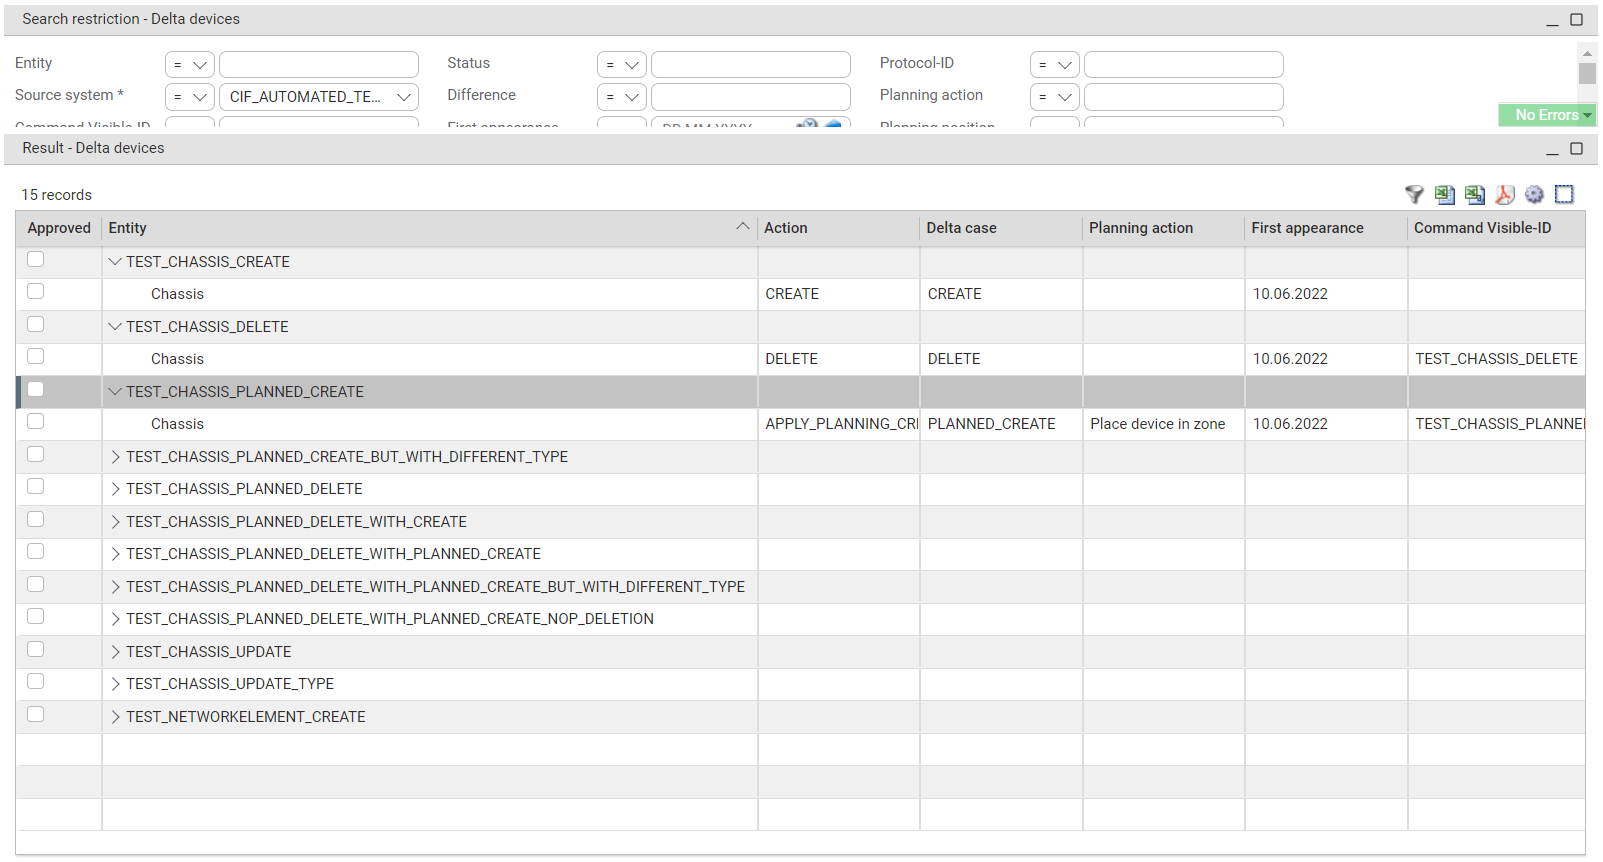
\includegraphics[width=\textwidth]{deltatable-screenshot.png}
    \caption{Deltatabelle nach erfolgreicher Testdatengenerierung und Deltaberechnung}
\end{figure}

\subsection{Dokumentation der Ergebnisse}\label{subsec:documentationChassis}
Es ist von großer Wichtigkeit, das Projekt anschaulich zu dokumentieren, damit ein einfaches Verständnis des Codes ermöglicht wird. Hierdurch kann eine bessere Wartbarkeit und Skalierbarkeit der Datengenerierung gewährleistet werden, auch, wenn das Projekt eventuell von anderen Entwickler*innen übernommen wird. Die Dokumentation der automatischen Testdatengenerierung findet daher ausführlich in der \textit{Readme}-Datei des Projekts \enquote{CIF Automated Tests} statt. Diese wird standardmäßig in der Online-Übersicht des Repository des Projekts angezeigt und kann so jederzeit gelesen werden. Sowohl die bereits umgesetzten Entitäten werden aufgelistet als auch die Konfigurationsdateien erläutert, sodass diese einfach angepasst werden können. Weiterhin wird auf Möglichkeiten zur Erweiterung der Datengenerierung eingegangen und eine kurze Anleitung zum Setup von Testdaten gegeben. Ein Ausschnitt der \textit{Readme}-Datei ist in der folgenden Abbildung einzusehen.

\begin{figure}[h]
    \centering
    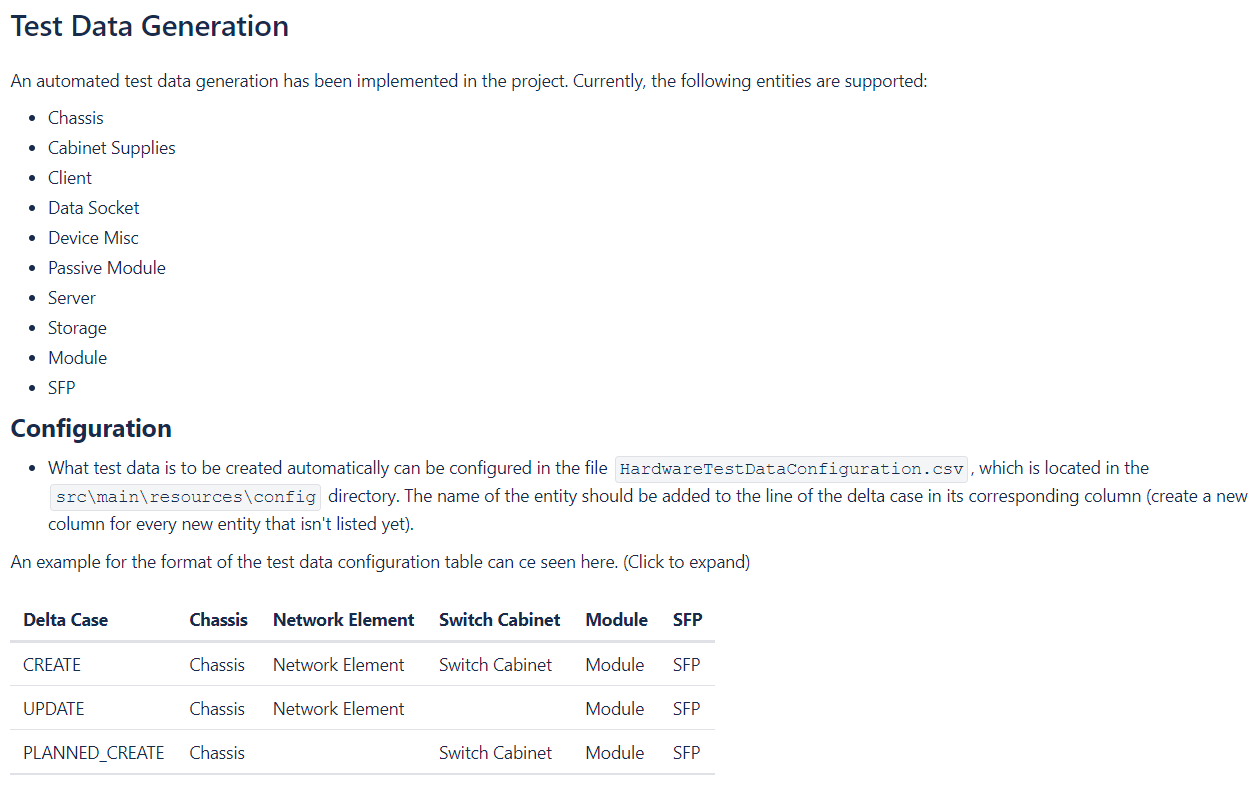
\includegraphics[width=\textwidth]{readme.png}
    \caption[Ausschnitt der \textit{Readme}-Datei]{Ausschnitt der \textit{Readme}-Datei in Online-Darstellung\footnotemark}
\end{figure}
\footnotetext{Die Abbildung wurde zu einem späteren Zeitpunkt erstellt, sodass schon mehrere Entitäten als implementiert angezeigt werden.}

\section{Erweiterung der Testdatengenerierung für Subequipment-Entitäten am Beispiel der Modules}\label{sec:tdgmodule}
Mit der korrekten Erkennung aller definierten Deltafälle für die von der automatischen Testdatengenerierung erstellten Chassis ist ein erstes Proof of Concept des Projekts erfolgreich abgeschlossen. Seit der Implementierung läuft die Datengenerierung bei den über \textit{Jenkins} ausgeführten automatisierten Tests mit und generiert zuverlässig Testdaten für die Tests der Chassis. Dies soll im nächsten großen Schritt jedoch auf weitere, komplexere Entitäten ausgeweitet werden. Konkret sollen Testdaten für sogenannte \enquote{Subequipments} generiert werden. Dies sind Entitäten, welche in andere Entitäten - zumeist sind dies Equipments wie Chassis - platziert werden. Um ein Testobjekt für eine Subequipment-Entität zu generieren, muss also zuvor immer auch erst ein hierfür vorgesehenes Equipment-Objekt als Vorbedingung generiert werden. Beispielhaft für Subequipment-Entitäten wird die Entität Module betrachtet und als Vorbedingung die bereits bekannte Equipment-Entität Chassis verwendet.

Das Vorgehen zum Generieren von Daten für Modules ist grundsätzlich gleich wie bei den bereits im vorherigen Kapitel ausführlich erläuterten Chassis. Lediglich einige Zwischenschritte müssen für die Modules erfolgen, welche für die Chassis nicht benötigt wurden. Es soll in den folgenden Unterkapiteln daher nur auf diese größeren Neuerungen eingegangen werden. Zwar unterscheiden sich Modules von Chassis auch maßgeblich in ihren Attributen, jedoch ändert dies nichts an Herangehensweises wie dem Abfragen dieser Attribute oder der Erstellung von Basisobjekten. Nicht explizit erklärte Vorgänge können daher als analog zu den für die Chassis geltenden Vorgängen angenommen werden.

\subsection{Das Factory Method Pattern}\label{subsec:factoryMethod}
Die Erweiterung der Datengenerierung zur Unterstützung von Modules bedarf größerer Anpassungen im Code, da einige neue Funktionalitäten zum Finden und zur Generierung von kompatiblen Chassis als Vorbedingung hinzugefügt werden müssen. Es können nicht einfach beliebige Chassis für beliebige Modules verwendet werden, da die Slots der Chassis, in welche Modules platziert werden, fest definierte Module-Kompatibilitäten besitzen. Es ist also nicht möglich, einfach über die schon für die Chassis implementierte Datengenerierung noch weitere Chassis für sämtliche Module-Deltafälle zu generieren. 

Theoretisch erlaubt \textit{Command} es, beliebigen Chassis Slot-Kompatibilitäten für Module hinzuzufügen. Jedoch widerspricht diese Herangehensweise der in Kapitel \ref{sec:anforderungen} erarbeiteten Anforderung, wonach die zu testende Instanz von den ausgführten Tests möglichst nicht dauerhaft verändert werden soll. Das Hinzufügen von Slot-Kompatibilitäten führt direkt Änderungen an Geräte-Masterdaten auf der zu testenden Instanz durch und lässt so Module-Chassis-Kombinationen zu, die der realen Welt eventuell nicht entsprechen. Selbst wenn die Kompatibilität nach den Tests wieder entfernt wird, besteht die Gefahr, dass zwischenzeitlich auf der Instanz gearbeitet wird und so verfälschte Masterdaten zum Einsatz kommen. Es wird also davon abgesehen, Änderungen an Masterdaten auf einer Instanz durchzuführen, sodass für einen ausgewählten Module-Typen tatsächlich kompatible Chassis gesucht werden müssen.

Um mit diesen und künftig nötigen weiteren Vorgehensschritten die bestehende Klasse \textit{DataGenerator} nicht immer mehr aufzublähen, wird für die Subequipment-Entitäten wie die Modules eine eigene \textit{DataGenerator}-Klasse implementiert. Hierbei kommt das sogenannte \enquote{Factory Method Pattern} zum Einsatz.

Das Factory Method Pattern, manchmal auch nur als Factory Pattern oder Simple Factory Pattern bezeichnet, ist ein Software Design Pattern zum Instanziieren von bestimmten Subklassen einer Superklasse, ohne dass der Aufrufer weiß, welche Subklasse genau instanziiert wird. \cite[S. 168]{metsker:2006} \cite[S. 22]{stelting:2002} Bei diesem Pattern wird kein direkter Konstruktor aufgerufen. Die Entscheidung, welche Subklasse instanziiert wird, fällt stattdessen eine Methode in einer sogenannten \enquote{Factory-Klasse} anhand des ihr übergebenen Inputs und liefert ein Objekt der korrekten Subklasse zurück. \cite[S. 19f.]{cooper:2000}

Im Fall der Datengenerierung bedeutet dies, dass anhand des Entitätsnamens entschieden wird, welche Subklasse der nun als abstrakte Superklasse definierten \textit{DataGenerator}-Klasse zu instanziieren ist. Das Objekt kann also je nach dem, welcher Entitätsgruppe die betrachtete Entität angehört, vom Typ \textit{EquipmentDataGenerator} oder vom Typ \textit{SubequipmentDataGenerator} sein. Der das Objekt anfordernden Methode in der Klasse \textit{DataGeneratorSteps} ist dies egal, da sämtliche \textit{DataGenerator}-Klassen dieselben Methoden anbieten und sich lediglich in ihrer konkreten Implementierung unterscheiden. Diese Herangehensweise erlaubt es auch, flexibel und relativ unkompliziert neue Varianten von \textit{DataGenerator} für weitere Entitäten hinzuzufügen. Es muss lediglich in der Factory-Klasse, welche in diesem Fall \textit{DataGeneratorFactory} genannt wird, die entsprechende Logik hinzugefügt werden, sodass für die neue Entität die korrekte Subklasse instanziiert und zurückgegeben wird. Das auf der nächsten Seite folgende Klassendiagramm soll den Aufbau der \enquote{Datengenerierungs-Factory} weiter verdeutlichen. Es ist anzumerken, dass die von der abstrakten Klasse \textit{DataGenerator} vererbten Methoden der Übersichtlichkeit halber in den Subklassen nicht aufgeführt wurden.

\begin{figure}[htp]
    \centering
    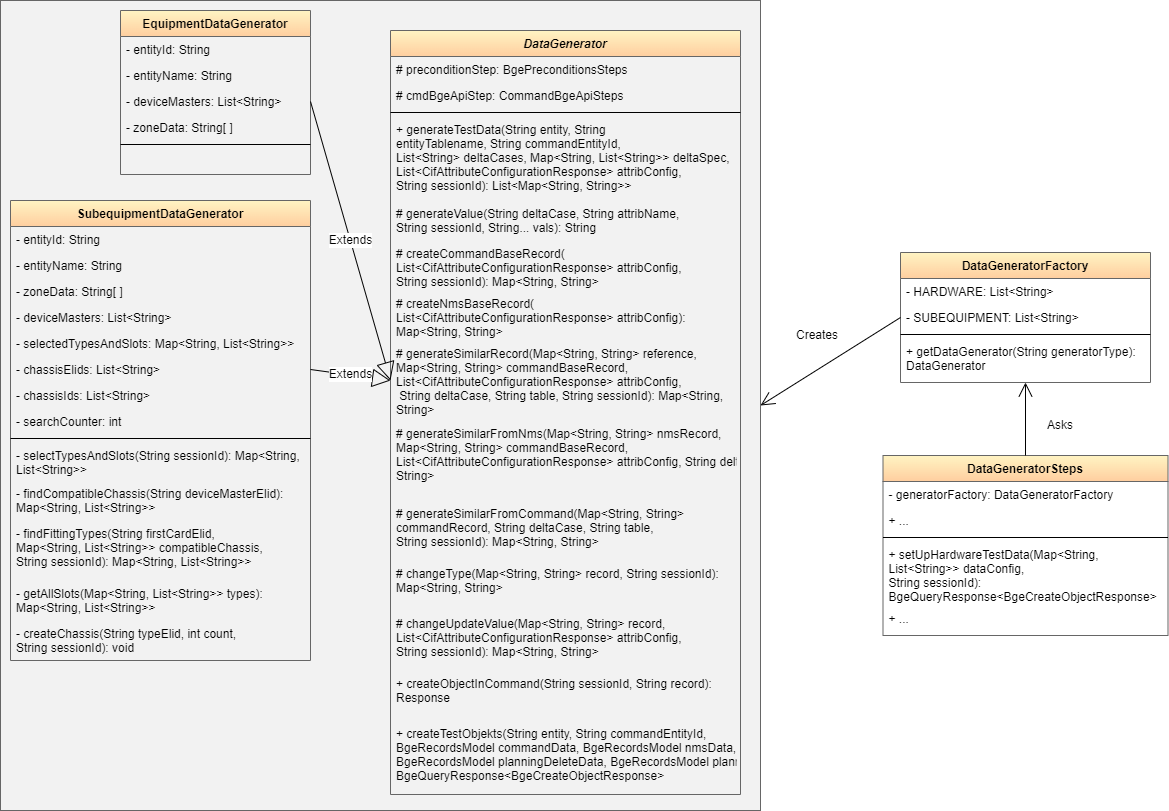
\includegraphics[width=.9\textheight, angle=90]{tdg_factory_method_class_diagram.drawio.png}
    \caption{Klassendiagramm des Factory Method Patterns im Projekt}
\end{figure}

\newpage
\subsection{Finden von kompatiblen Module-Chassis-Paaren}\label{subsec:findCompatibleTypes}
Modules können nicht für sich alleinstehend in \textit{Command} erstellt werden, sondern brauchen eine Art Elterngerät, in welches sie platziert werden. Um Testdaten für das Module zu generieren, müssen also zunächst kompatible Chassis gesucht werden. Diese Suche wird vor dem Erstellen der Basisobjekte durchgeführt, da das \textit{Command}-Basisobjekt für das Module bei seiner Erstellung in \textit{Command} platziert wird und dadurch dort bereits ein Chassis vorhanden sein muss.

Das Finden von kompatiblen Typen verläuft größtenteils über Datenbankabfragen, da die benötigten Informationen nicht ohne Weiteres über die \ac{BGE} abrufbar sind. Nach der Abfrage der auf der Testinstanz möglichen Module Device Master wird zufällig einer dieser Typen als primärer Module-Typ ausgewählt. Aus der Datenbanktabelle \textit{STCSPC\_CHASSIS\_SLOT} können dann mit der \ac{Elid} dieses Typs als Sucheinschränkung sämtliche Chassis-Typen ausgewählt werden, welche das Module unterstützen. Zusätzlich hierzu werden für jedes prinzipiell kompatible Chassis die Namen der Slots gespeichert, in die das Module passt. Ein kompatibles Chassis kann beispielsweise auch zehn Slots besitzen, von welchen nur einer tatsächlich für das Module geeignet ist. Aus dieser Liste von möglichen Chassis mit ihren kompatiblen Slots wird nun ein Typ ausgewählt, welcher in mindestens einem Slot mindestens zwei verschiedene Module-Typen unterstützt. Dies ist notwendig für Deltafälle, die auf Typunterschieden zwischen \ac{NMS} und \textit{Command} basieren.

Wurde ein Chassis gefunden, welches einen solchen Slot besitzt, wird aus den für den gefundenen Slot passenden Module-Typen ein sekundärer Typ ausgewählt und die \ac{Elid}s und Typnamen für sämtliche ausgewählte Typen, sowohl Module als auch Chassis, gespeichert. Den letzten Schritt der Chassis-Module-Suche stellt die Sammlung und Speicherung aller Slotnamen und Slotnummern des ausgewählten Chassis-Typs dar, welche sowohl den primären als auch den sekundären Module-Typ unterstützen. So können später bei der Generierung der Testobjekte die passenden Slots einfach zugeordnet werden.

Die Liste der verfügbaren Slots pro Chassis ermöglicht es, genau auszurechnen, wie viele Chassis benötigt werden, um alle Module unterzubringen. Um die Performance zu verbessern und Ressourcen zu sparen, werden nur so viele Chassis generiert, wie auch tatsächlich nötig sind. Dies entspricht auch den aufgestellten Anforderungen in Kapitel \ref{sec:anforderungen}.

\subsection{Erweiterung der \textit{generateValue()}-Methode mit Java-\textit{Varargs}}\label{subsec:varargs}
Bevor die Basisobjekte für die Modules erstellt werden können, müssen die Vorbedingungen erfüllt, also die Chassis erstellt werden. Hierfür wird die bestehende \textit{generateValue()}-Methode wiederverwendet. Da diese allerdings standardmäßig Werte für Attribute wie \textit{visibleId} nach einem festen Schema aus dem Entitätsnamen und dem Deltafall der Hauptentität, also dem Module, zusammensetzt, würden so Chassis mit irreführenden \textit{visibleId}-Werten erstellt werden. Um dies zu umgehen, wird die \textit{generateValue()}-Methode mit sogenannte \textit{Varargs} erweitert. \textit{Varargs} in Java stellen eine Möglichkeit dar, Methoden um eine variable Anzahl von Parametern zu erweitern, welche dann zu einem Array zusammengefasst werden. \cite[S. 11]{naftalin:2006} In diesem Anwendungsfall können so der Methode \textit{generateValue()} bei Bedarf ein oder mehrere vordefinierte Werte übergeben werden, die zur Wertegenerierung mitverwendet werden. Für \textit{visibleId}-Werte der für die Modules benötigten Chassis wird der Methode konkret mitgeteilt, dass es sich bei der betrachteten Entität um Chassis und nicht Modules handelt, sodass ein sprechender \textit{visibleId}-Wert generiert werden kann.

\begin{lstlisting}[caption=Einsatz von \textit{Varargs} in der \textit{generateValue()}-Methode, label=varagsCode,style=Javastyle]
@Override
protected String generateValue(String deltaCase, String attribName, String sessionId, String... vals) throws IOException {
    String out = "";
    
    if (attribName.equals("visibleId")) {
        out = DataGeneratorUtils.generateVisibleId((vals.length > 0 ? vals[1] : this.entityName), deltaCase);
    }
    ...
    return out;
}
\end{lstlisting}

\textit{Varargs} werden über die Syntax \colorbox{background}{\lstinline{...}} dargestellt und müssen immer als letzter Parameter im Methodenkopf stehen. Im Codebeispiel wird überprüft, ob das \textit{Varargs}-Array einen Wert enthält. Ist dies der Fall, so wird dieser Wert zur Generierung einer \textit{visibleId} übergeben anstatt des \textit{entityName}, da diese Variable im Fall der Chassis, welche als Vorbedingungen für Modules erstellt werden, den Wert \enquote{Module} enthalten würde.

Bei der Erweiterung der von allen \textit{DataGenerator}-Subklassen implementierten Methode \textit{generateValue()} zeigt sich gut ein Nachteil des gewählten Factory Method Patterns. Wenn eine Änderung an einer vererbten Methode gemacht wird, muss diese Änderung bei allen Klassen durchgeführt werden, die diese Methode implementieren. In größeren Projekten kann dies durchaus einen erheblichen Aufwand bedeuten. Für den Umfang der automatischen Testdatengenerierung im \ac{CIF} ist dieser Aufwand allerdings überschaubar.

\section{Erstellen eines Konzepts zur Testdatengenerierung für Telco-Entitäten}\label{sec:tdgtelco}
Subequipment-Entitäten stellen im Vergleich zu den primitiven Equipment-Entitäten eine höhere Komplexitätsstufe dar, da sie auf letzteren aufbauen. Theoretisch kann dies noch weitergeführt werden; Subequipments können sogar in anderen Subequipments platziert werden. Die Entitäten folgen also einer Hierarchie, wonach bei der nächsthöheren Stufe immer alle Objekte der tieferen Stufen als Vorbedingung benötigt werden. Ähnlich verhält es sich bei den Telco-Entitäten, also Entitäten, welche Telekommunikationsinfrastrukturen abbilden. Deren Hierarchie ist wie folgt aufgebaut:

\begin{itemize}
    \item Network Element oder Device (beispielsweise Chassis)
    \item Logical Ports: erlauben das logische Verbinden von Geräten
    \begin{itemize}
        \item Typ 2: wird auf Chassis platziert
        \item Typ 3: wird auf Network Element platziert
    \end{itemize}
    \item Bearer: verbindet zwei Logical Ports und bietet Services Ressourcen wie Bandbreite oder Frequenz an
    \item Services: werden auf Bearer gesetzt und nutzen deren Ressourcen
    \begin{itemize}
        \item Path: Verbindung zwischen zwei Punkten, geroutet
        \item Unrouted Path: Verbindung zwischen zwei Punkten, ungeroutet (Route ist irrelevant)
        \item Unrouted Multipoint: Verbindung von mehreren Punkten zu einer Art Netz, ungeroutet (Routen im Netz sind irrelevant)
    \end{itemize}
\end{itemize}

Auch für diese soll eine automatische Datengenerierung konzeptioniert und realisiert werden. In Anbetracht des limitierten Zeitumfangs dieser Arbeit konnte die Realisierung für die Telco-Entitäten nicht mehr durchgeführt werden, jedoch wurde ein ausführliches schriftliches Konzept erstellt, welches auch anderen Entwickler*innen eine Fortführung der Arbeit an der automatischen Testdatengenerierung in Zukunft ermöglicht. Ein Ausschnitt dieses Konzepts ist in Anhang \nameref{app:telcoKonzept} einzusehen.